\newpage

%---------------------------------------------------------------------------------
% Approach
%---------------------------------------------------------------------------------

\section{Approach}

\quad In this section, we will go on to describe our approach of modelling American Football as a Cyber-physical system. We'll talk about some of the simplifications we make as well as our design choices.

\subsection{Simplifying the Model}

\quad Either football team has 11 players. It can be difficult to hardcode all these "robots", or players, so we seek to make a few simplifications. We first reduce our number of players, then restrict the particular play they're running, reduce the dimensions, and re-frame things to focus on quarterback safety.

\subsubsection{Categorical Players}

\quad We will reduce our model to a total of 6 robots, or "player categories". We will have a Quarterback, Offensive Lineman, Defensive Lineman, Wide Receiver, and Linebacker. The Quarterback still is the same as in normal football, since there is one Quarterback on the offensive team. For the linemen (OL and DL), we will leverage the ideas from our related works section and view the various linemen on a football team as a "collective". Namely, there will be one robot who symbolizes the collective of the Offensive Line, and one for the Defensive Line. In real football, these linemen are in a relatively close position performing very similar actions, so viewing them as a collective will suffice for our model. We will design our singular Offensive Lineman and Defensive Lineman in such a way that is likely more "dangerous" than what we might expect from reality in order to be conservative with our model. Finally, for the Wide Receiver and Linebacker, we will only consider one these "pairings". In real football, there will be a few different Wide Receivers to pass to, given the Quarterback various options to make. By reducing it to one "pairing", we limit the Quarterback's possible options. It follows that if the Quarterback is able to safely pass with just one option, he only become "safer" with more options to pass to.

\subsubsection{Hail Mary}

\quad There are various plays in football which involve certain players running certain routes and such. This can lead to some undesired complexity, so for our model, we will pick a simple football play known as “Hail Mary.” We see that there are 5 Wide Receivers (WR), each with a forward arrow representing the path they will follow. Their goal is to run forward and catch the ball if it is thrown to them while avoiding contact from the Linebacker (LB). The dots with a seemingly inverted-T shaped root to them and are aggregated in the center represent our 5 Offensive Linemen (OL), whose goal is to protect the Quarterback (QB) from the Defensive Line (DL, not in picture). Finally, the last dot towards the bottom that is seemingly being protected, is the QB. Since we have simplified our number of players as described above, we will not have this wide receivers in our model. The way we use a Hail Mary plan is to hard-code a route for our Wide Receiver to travel along. In a Hail Mary play, he will only move forward, so this simplifes the Ordinary Differential Equation we will use to model his movement. Hard-coding the WR's path like this is still accurate the real life football since the Quarterback decides the play that is being run. In a sense, the QB decides the ODE's of the offensive players. \\

\begin{figure}[htp]
    \centering
    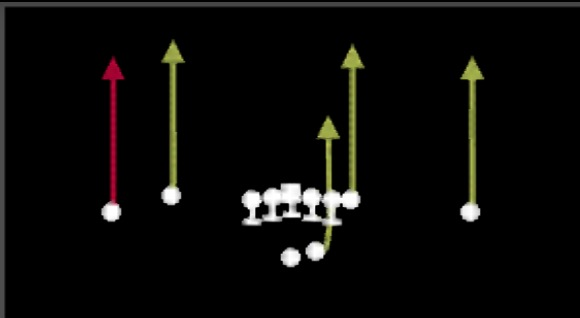
\includegraphics[width=7cm]{figure/hailMary.png}
    \caption{A depiction of a Hail Mary Pass in video game NFL Mobile.}
\end{figure}

\subsubsection{One Dimension}


Len 
- Actually a lil confused on this maybe need megha help
- The plays on a football field for the haily mary play is roughly symmetric
- If we can guarantee for what's in front of us, shouldn't be too hard to do left and right
  as well end up having more freedom to move and maneouvar ins afe was

\subsubsection{The Equivalence of Openness and Passing}

\quad One assumption that we will make is that openness is equivalent to passing. The main problem we seek to discuss is can our Quarterback safely pass the ball? As such, we will assume that, when presented with the opportunity, our Quarterback will pass the ball to the Wide Receiver as soon as he becomes open. This means that our system has successfully protected the Quarterback for the necessary duration. As such, we will not worry about the physical act of passing for our model since we are focusing on the safety of the Quarterback. Though it is a bit unrealistic to say that the Quarterback can instantaneously pass the ball to the wide receiver, we will use this assumption to simplify our model and put a larger focus on Quarterback safety. 


\subsection{Realistic Magnitudes}

\quad Some things we will need to keep in mind for our model are realistic conditions. We are able to set these values and not leave them up to further generality because football is "defined" to have some of these constraints. The first will be the dimensions of the football field, and thne the speeds of the players.

The football field’s dimensions are 160 feet by 300 feet. If we consider the football field to be on a coordinate plane, with the units being in feet, we will let the lower left corner be at the point (0, 0), the upper right corner be at (160, 300), and the center be at (80, 150). We will also consider the scenario where the Quarterback starts at this halfway point in our model.

We gathered data from the NFL Combine (an event where prospective football players participate in various events to demonstrate their physical abilities) to determine appropriate speeds for our various players [1]. A 40 yard dash time is how long it takes a player to run 120 feet at a full sprint. Note that quarterbacks usually move slowly since they need to be in a stable position to throw far distances. We model this by setting the QB's speed to the average pace at which a human walks. To get their speed in feet per second we do $120 \div dash$. Since we have this notion of a categorical player, we can reduce each player to their positions and find statistics per positions. 

\begin{center}
\begin{tabular}{ |c|c|c| } 
 \hline
 \textbf{Position}\footnotemark & \textbf{40-yard Dash Time} & \textbf{Feet Per Second} \\ 
 \hline
 Quarterback & -- & 4.6 \\ 
 Wide Receiver & 4.48 & 26.79 \\ 
 Linebacker & 4.76 & 25.21 \\ 
 Defensive Lineman & 5.06 & 23.71 \\ 
 Offensive Lineman & 5.34 & 22.47 \\ 
 \hline
\end{tabular}
\end{center}

\footnotetext{Here we refer to specifically the Inside Linebacker. Defensive Lineman can also be called Defensive Tackles. finally, The Offensive Lineman is the average of the Offensive Guard and Tackle.}

\subsection{The Players}

\quad We will break the system down into its smaller subparts, by first examining how the Offensive and Defensive Lines work. To simplify the system, we will consider the Offensive Line and Defensive Line as their own single lines that move as a unit rather than individual players. In real football, the players might struggle to break past one another. For our model, we will simplify this by saying that the Defensive Line slowly approaches the Quarterback.

\subsubsection{Linemen Collision}
\quad  In football, there is no fixed rule as to where the Offensive and Defensive Lines need to start exactly. The only constraint is that the Offensive Line starts in front of the Quarterback on one side of the Line of Scrimmage and the Defensive Line starts on the other side of the Line of Scrimmage as visible in the visual to the right. We will be viewing the football field from the perspective of the offense. \\

Note that the Offensive Line’s duty is to protect the Quarterback and the Defensive Line’s goal is to tackle the quarterback before he throws the ball. Therefore the Defensive Line travels toward the quarterback, which is the negative direction on the y-axis ($dy_D$). On the other hand, the Offensive Line travels away from the Quarterback, which means they travel in the positive direction on the y-axis ($dy_A$). To simplify the model, we consider that both of the lines travel with a constant velocity before they collide. We visualize the velocities and directions of the two lines in the diagram to the right. \\

% Upload file to figures and change the \includegraphics to the name of file, update caption
\begin{figure}[htp]
    \centering
    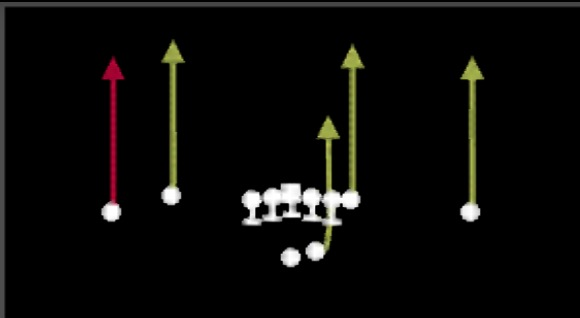
\includegraphics[width=7cm]{figure/hailMary.png}
    \caption{Change the wording so it's not "the image on the right". Rather Figure X}
\end{figure}

The Defensive Line, represented by the red line, is moving with speed $vy_D$ in the direction $dy_D$, and the Offensive Line (blue) is moving with speed $vy_A$ in direction $dy_A$. Note that $vy_D$ and $vy_A$ are the magnitudes of the lines' velocities, and are therefore non-negative. \\
 

At the start of the play, the two lines will charge towards each other. However, once the two lines collide, they will move as one unit with the velocity being the sum of their initial velocities; this models a perfectly inelastic collision. The NFL Combine is an event where players compete in various athletic tests such as a 40-yard dash, vertical jump and more. We aggregate NFL Combine results for the 40-yard dash to derive an estimate of what each position's average speed might be. From these results, we see that Defensive Linemen are faster than Offensive Linemen across the National Football League; we model this by making the magnitude of the initial velocity of the Defensive Line greater than the magnitude of the velocity of the Offensive Line. Therefore, when the two lines collide, their velocities will counteract one another, effectively dampening the velocity of the Defensive line. One might think of this as two people pushing against one another, but one eventually dominating the other in terms of force, thus pushing them back. Taking into account the force of the Offensive and Defensive lines, we see that they will travel with a velocity that has a magnitude equivalent to half of the difference between the magnitudes of the initial Defensive and Offensive Line’s velocities. If we consider that the masses of the Offensive and Defensive Lines are the same, we know that this abides with the Principle of Momentum Conservation because of the following equations. \\

Let $m_A$ and $m_D$ be the masses of the Offensive and Defensive lines respectively, where $m_A = m_D = m$. Let $vy_{Ai}$ and $dy_{Ai}$ be the initial velocity (magnitude) and direction of the Offensive Line, $vy_{Di}$ and $dy_{Di}$ be the initial velocity (magnitude) and direction of the Defensive Line, and $vy_f$ and $dy_f$ be the final velocity and direction of both lines together after the collision. By the conservation of momentum, we have:
% Len: I changed this slightly because things are showing up weird on Overleaf
\begin{align*}
m_A \cdot vy_{Ai} \cdot dy_{Ai} + m_D \cdot vy_{Di} \cdot dy_{Ai} &= m_A \cdot vy_f \cdot dy_f + m_D \cdot vy_f \cdot dy_f \\
m(vy_{Ai} \cdot dy_{Ai} + vy_{Di} \cdot dy_{Ai}) &= 2 \cdot m \cdot vy_f \cdot dy_f & (m = m_A = m_D) \\
m(vy_{Ai} - vy_{Di}) &= 2 \cdot m \cdot vy_f \cdot dy_f & (vy_{Ai} = 1, vy_{Di} = -1) \\
vy_{Ai} - vy_{Di} &= 2 \cdot vy_f \cdot dy_f & (\text{eliminate m}) \\
\frac{vy_{Ai} - vy_{Di}}{2} &= -vy_f
\end{align*}

Since vyDi > vyAi (the Defensive Line is faster than the Offensive Line), we know that the left hand side has to be negative as (vyAi - vyDi)/2 < 0. Therefore, vyfdyf < 0, and vyf is a magnitude so it cannot be negative. Therefore, dyf = -1, and the direction is the same as the Defensive Line’s original direction. We have (vyAi - vyDi)/2 = -vyf . The progression of movement is shown in the following figure.

\subsubsection{The Quarterback}
\quad The next component of our system is the Quarterback. The Quarterback is a player that we must protect, and in order for the offense to have a winning strategy and remain safe, the Quarterback must not be tackled until he executes a pass. 

\subsubsection{Looking to Pass}

\quad The next component of our system is the Quarterback. The Quarterback is a player that we must protect from getting tackled by the Defensive Line. In our system, tackling is represented as the intersection of their y-coordinates. In order for the offense to have a winning strategy and remain safe, the Quarterback must not be tackled until he executes a pass. Therefore, this winning strategy depends on two things: the Quarterback’s ability to pass and his ability to stay away from the Defensive Line. 

The Quarterback’s ability to not get tackled is enabled by his ability to travel backwards away from the Defensive Line. Because the Quarterback travels at a speed faster than the dampened Defensive Line speed, we know his safety is ensured. Therefore, the only aspect remaining to ensure a successful run is whether the Wide Receiver can get open while all the players are still on the field. Our notion of the Wide Receiver being open is when he passes the y-direction of the Linebacker. This is possible when the Wide Receiver is slightly faster than the Linebacker, since the Linebacker starts ahead of the Wide Receiver.

We assume that the Quarterback can throw the ball whenever he needs to; however, in order for the pass to be successful, we HI! 

\subsubsection{Zone Defense}

Megha (Len double check)

\subsubsection{Man Defense}

Megha 